\subsection{2024/3/4 问题}
refine流程
\begin{itemize}
	\item 先将三角面保存投影到相机的归一化平面中,并且开启深度检测,将深度缓存提取出来获取三角面的深度图
	\item 在创建一张faceinfo的面信息图,面信息包括图元id、c值是$(1,0,0)、(0,1,0)、(0,0,1)$
	\item 在第二张图片中,重投影深度较小的像素值会写入到重投影图中。
	\item 基于重投影中,重投影深度比较小的点,计算一张深度梯度图
	\item 在两张途中ncc值较小的两个像素输出一个相关性(correlation)梯度值
	\item 顶点位置-(顶点三角面法向*梯度值)
\end{itemize}

\begin{figure}[h]
    \centering
    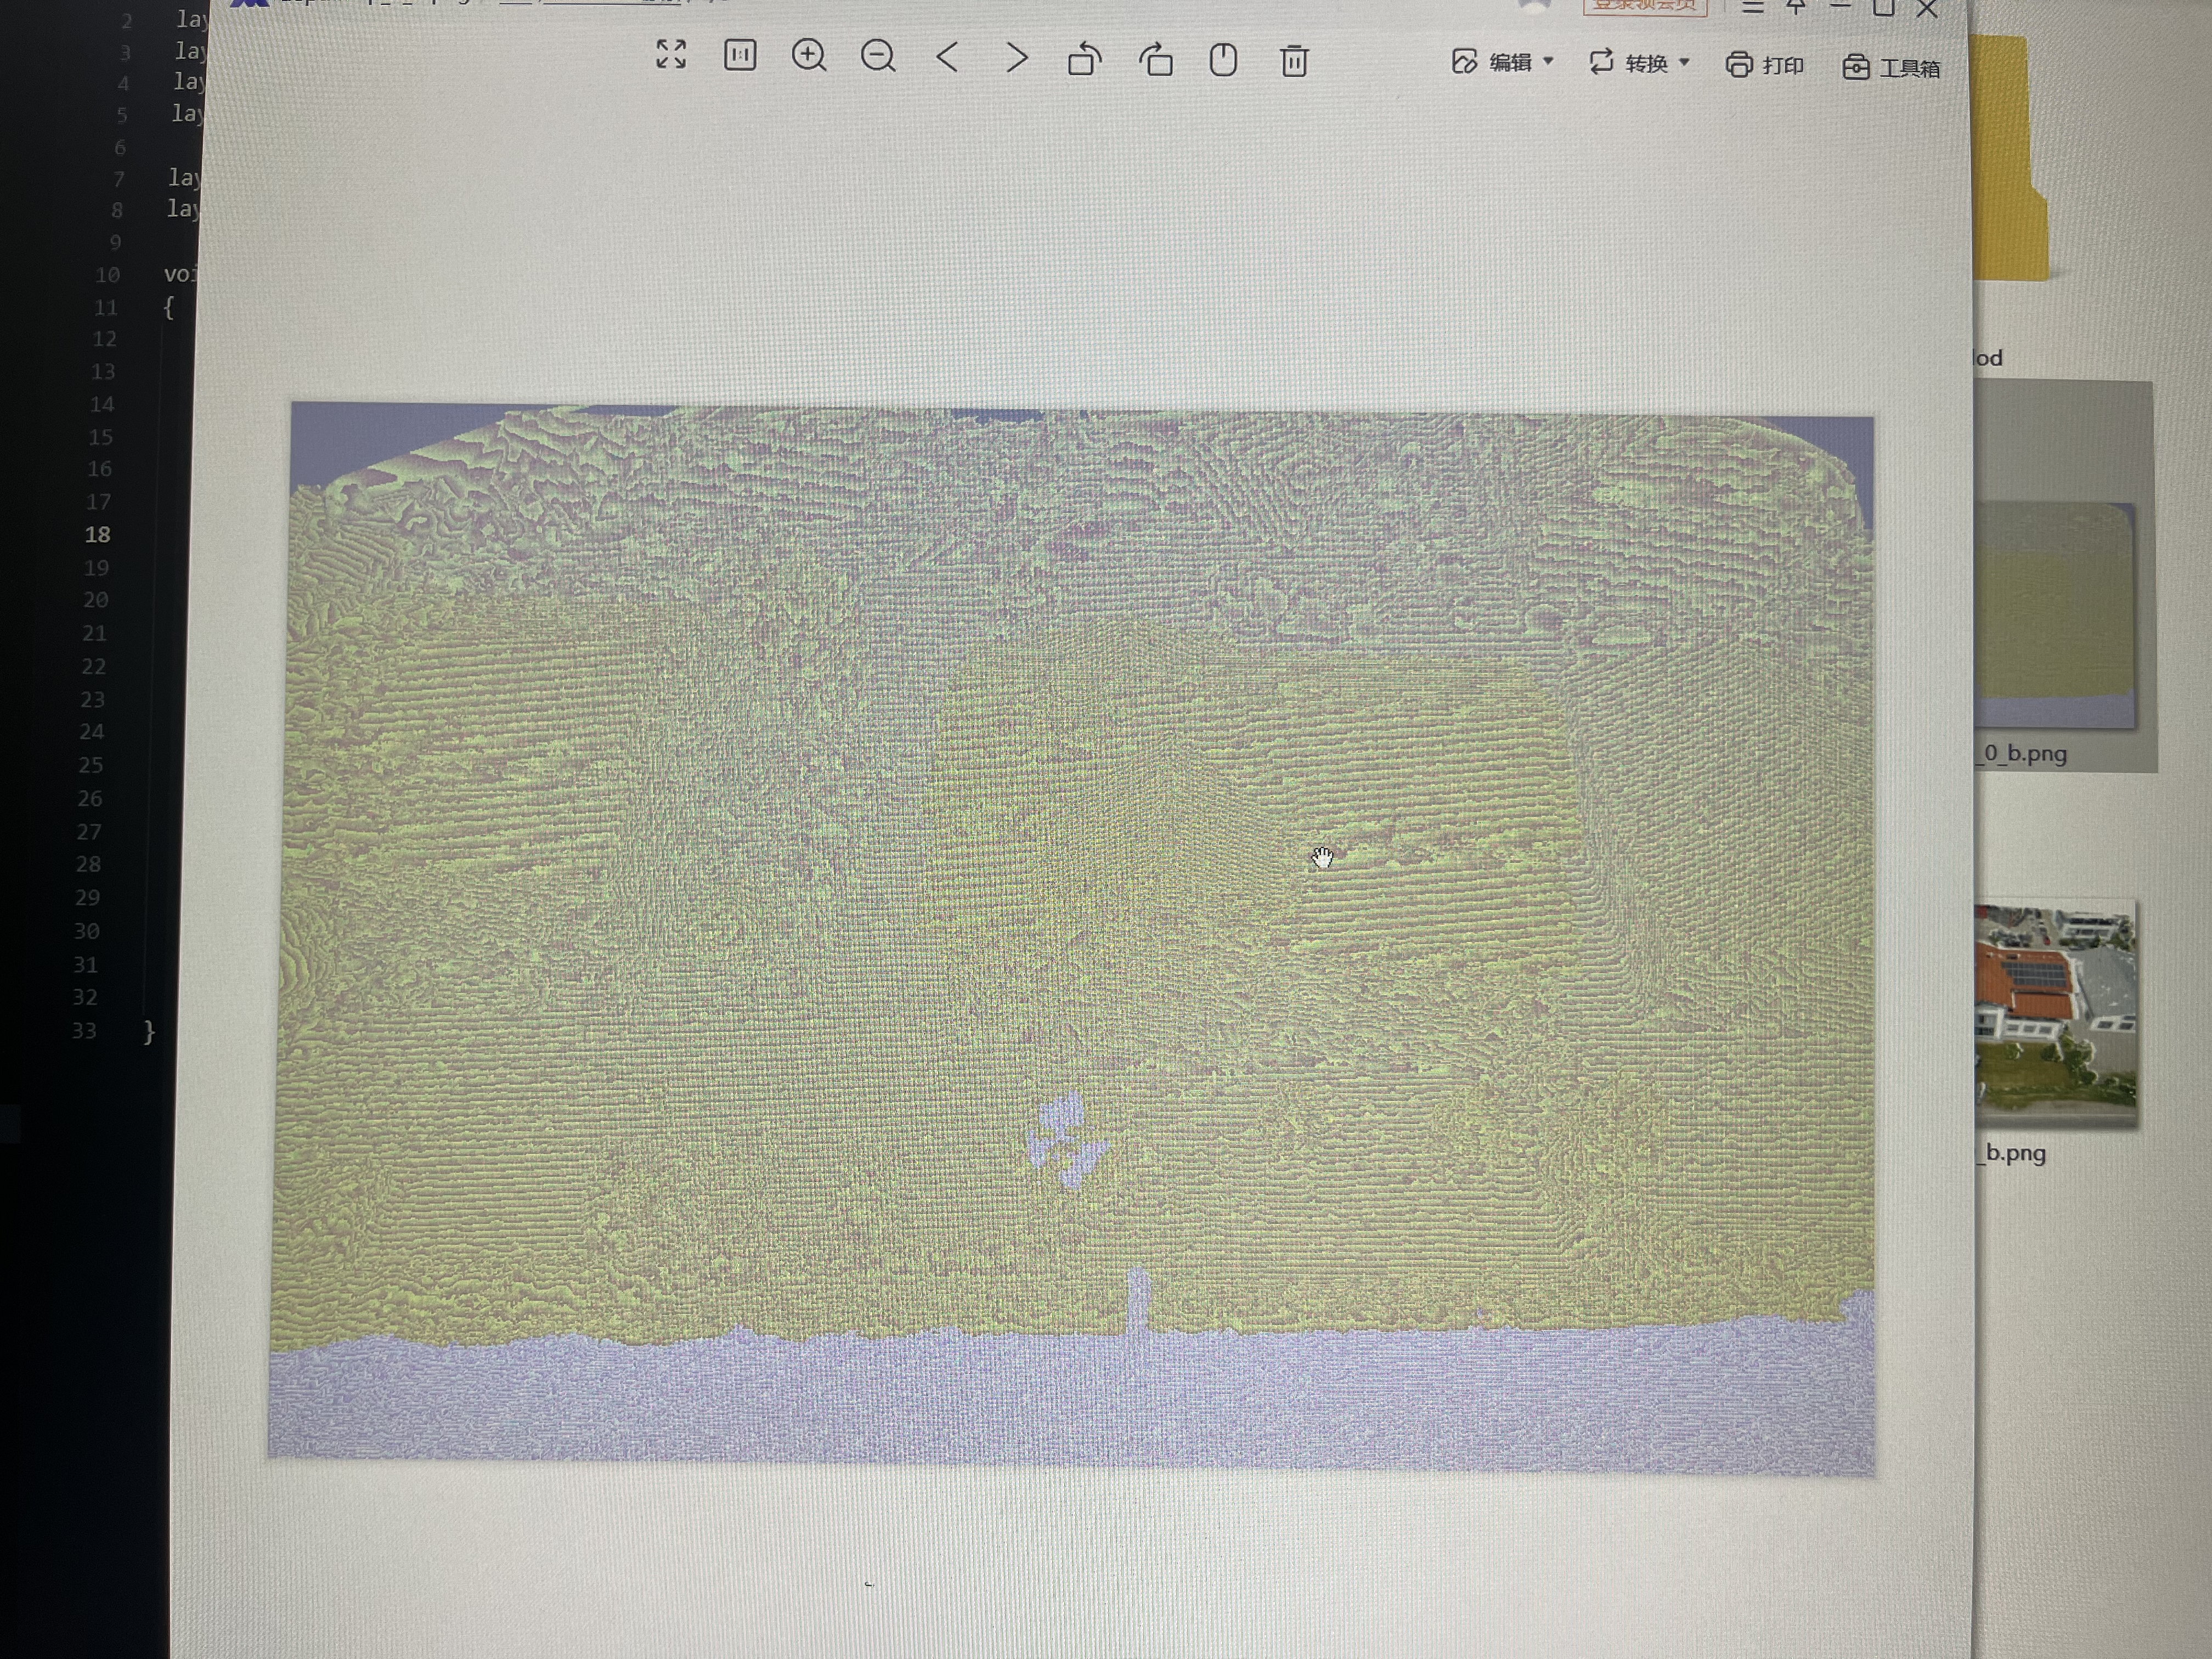
\includegraphics[height=5in]{depthmap.jpg}
    \caption{深度图}
\end{figure}

\begin{figure}[h]
    \centering
    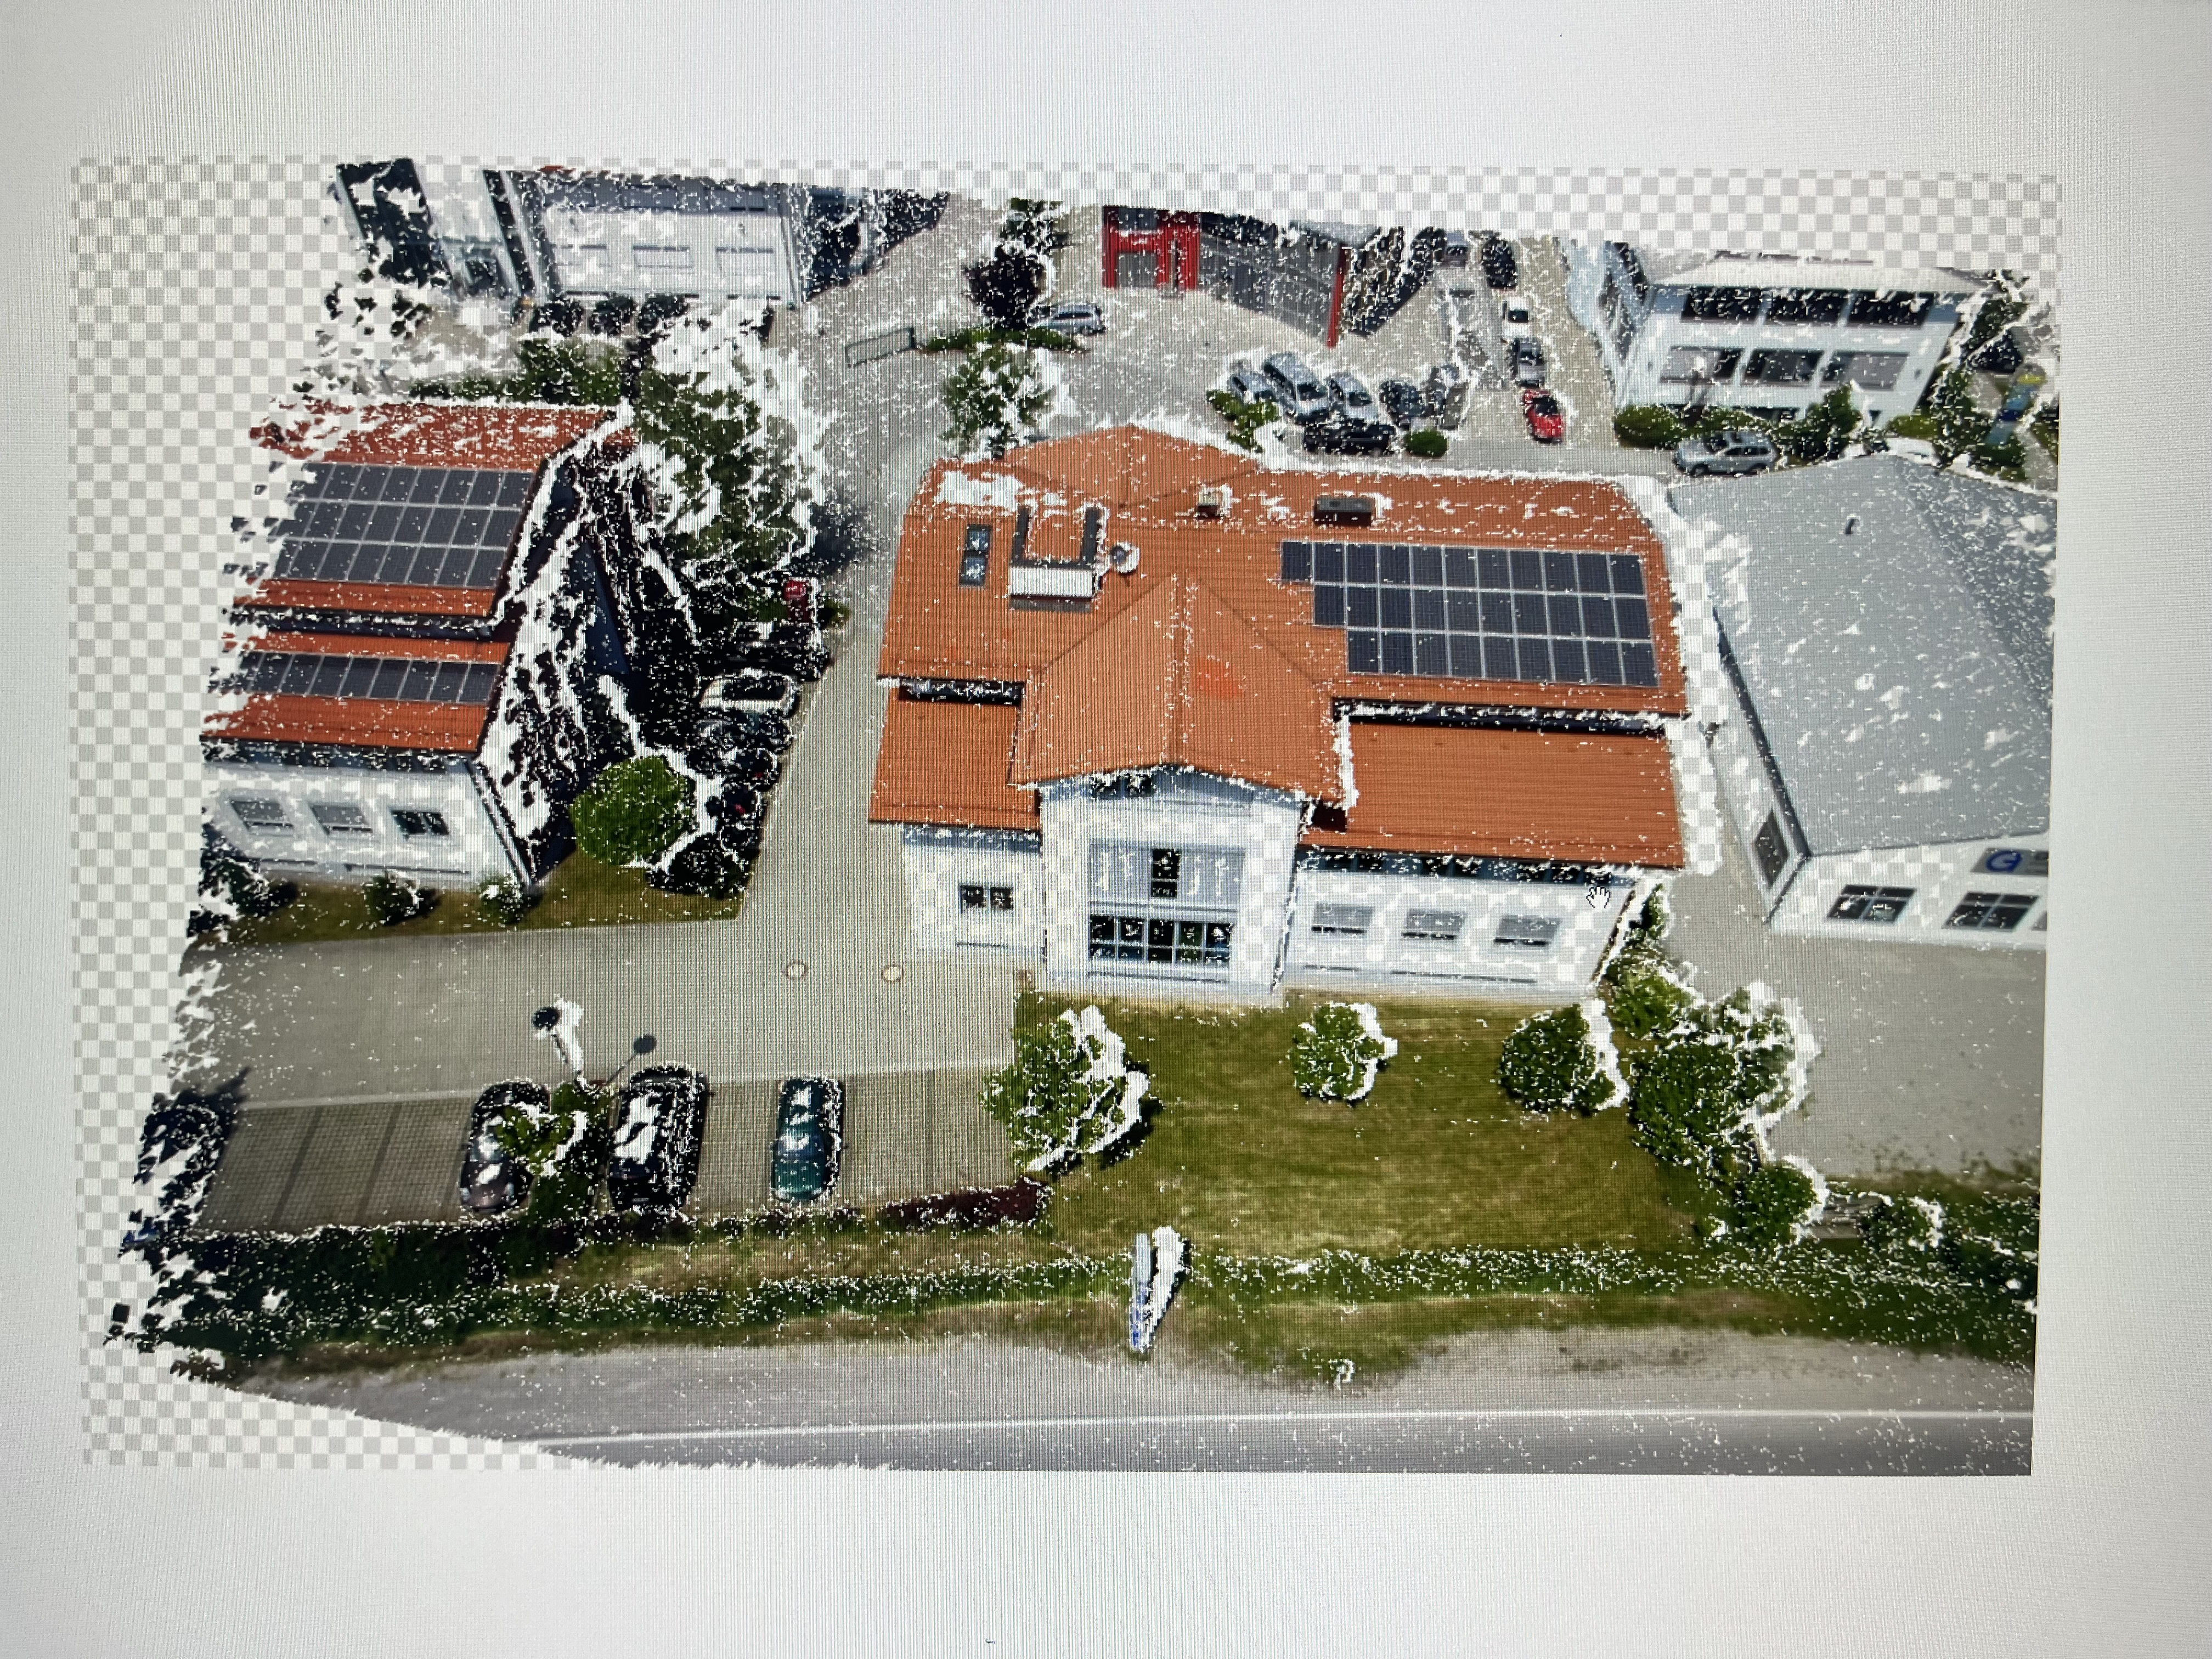
\includegraphics[height=5in]{reprojection.jpg}
    \caption{重投影}
\end{figure}

\begin{figure}[h]
    \centering
    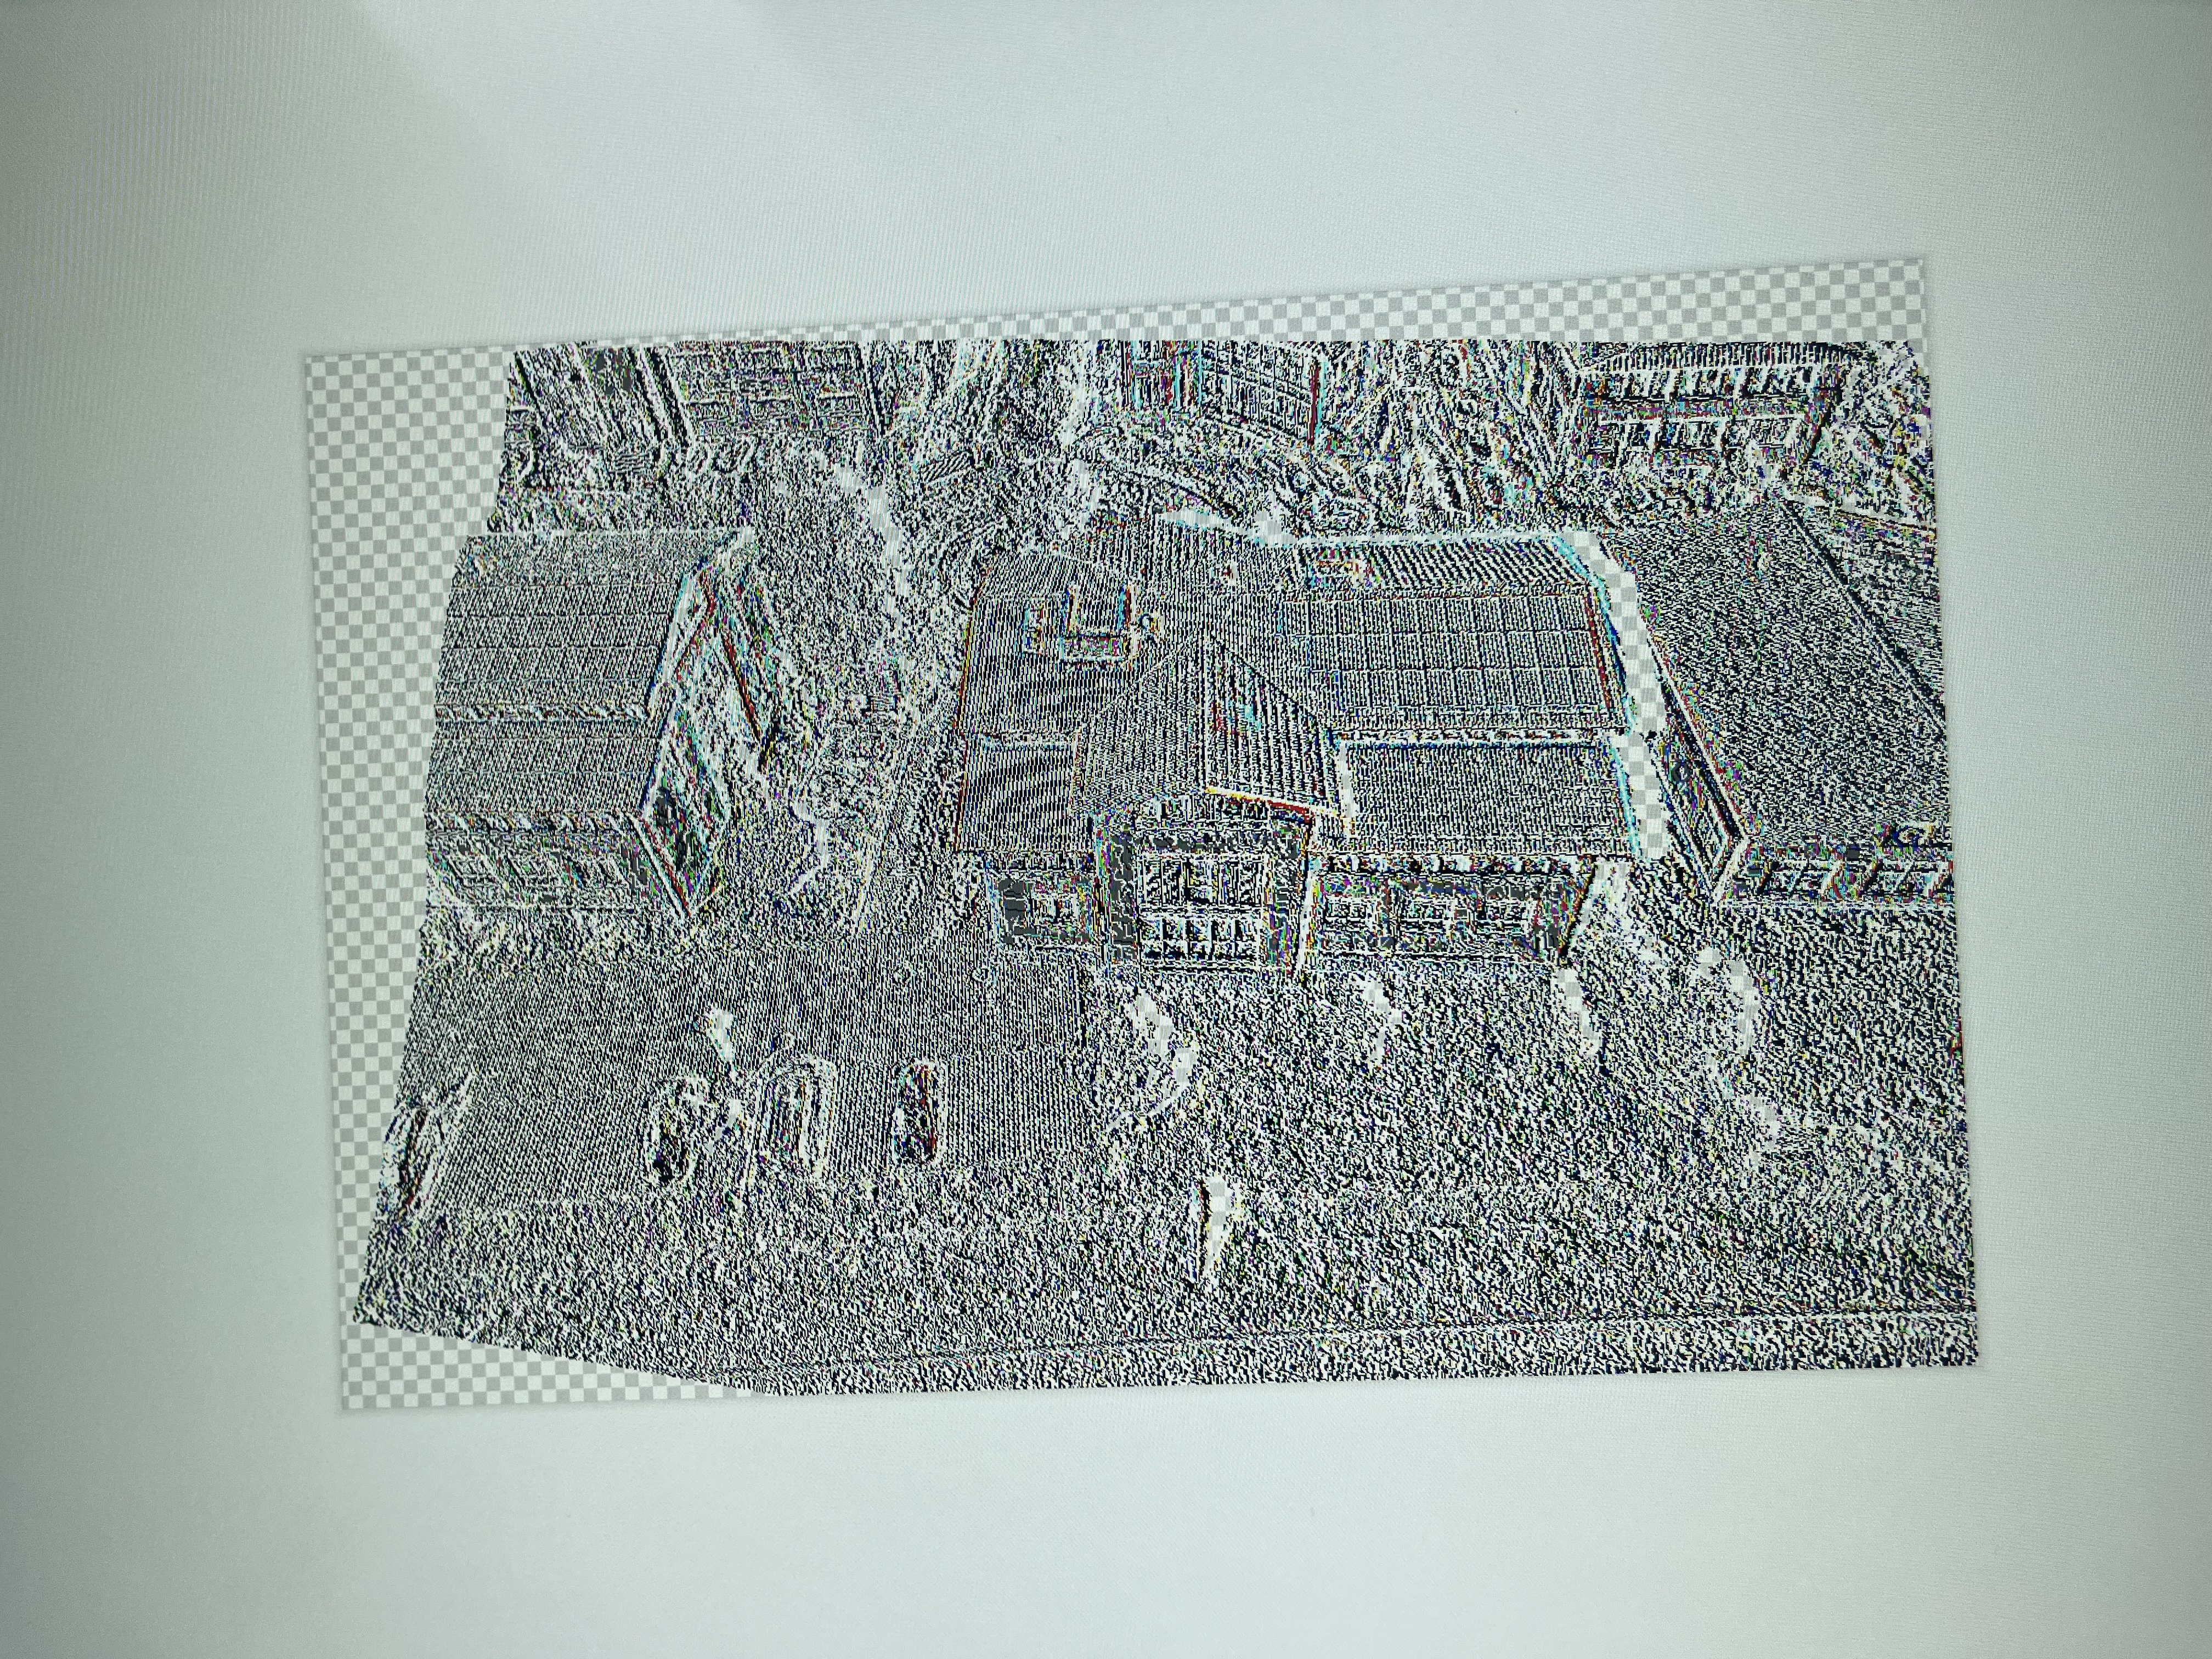
\includegraphics[height=5in]{variation.jpg}
    \caption{深度梯度}
\end{figure}

\begin{itemize}
	\item 什么是ProjectionVulkanMatrix矩阵,看起来好像是投影到相机归一化平面的矩阵
	\item 什么是TextureMatrix矩阵?
\end{itemize}

会议记要

密集匹配:平面扫掠+acmm

两相对用来rgb值或者计算灰度值

如果知道rgb会调用colorshader,如果是灰度图则调用grayshader

三相对是只有r通道。

隔几个像素计算深度值,不是逐像素的计算深度值。

相邻像素没有深度对应关系,acmm像素与像素之间是相关的。

三个线程:

\begin{itemize}
	\item 图像校正+图像金字塔创建(不做极线矫正)直接根据内外参数,计算单应矩阵。
	\item gpu平面扫掠密集匹配
	\item 保存密集点云
\end{itemize}

Densepair,正反做了两次校验,交叉校验,生成两张图像的深度。

会对深度做一次refine的操作,两张能回复出空间点云,相邻点(20个点)聚合成平面,基于平面知道这个点的法线,
将点基于法向进行移动,反投影到图像上,计算ncc最小的。反复计算,得到最小的ncc的点最终作为点的调整量。

将面的调整量会插值到顶点的调整量。平面上下分别取5个面,就有十个调整量,基于这是个位置,移动顶点,计算ncc,计算最小的ncc值作为最终的调整量。
只是单调一个点。

得到的密集匹配点最后进行聚类和平滑。

按距离采样间隔,将一点范围内的点降采样到最终的点。

Smooth是去外点(去噪点)。

我们的ncc是简化,是为了将除法操作去掉。


refine中会对ncc进行求导,如果加入几何一致性,需要求几何一致性导数。

会对一个空间进行平面均匀分割,对当前平面每个点进行投影到两个相对,如果两个相对的投影值的ncc值小于一定参数,当前点的深度会被保留。

聚类也对细杆有影响。


构网

构网openmvs的细节更多,mvs的细节较少。(细杆)

纯CPU

对空间进行权重计算,点和相机位置合成一个boundbox。

对空间进行的劳累四面体进行切割。从四面体中查找平面。找的方式是找零值面。


refine:

固定次数20次。mvs不是自适应没有终止条件。将分辨率不行,必须用原始分辨率。

refine的细杆呈现效果不好。

GPU加速

\begin{itemize}
	\item 快速:两个分辨率(1/4和1/2)
	\item 普通和精细:三个分辨率
\end{itemize}

2 、 1 、0
$\frac{1}{2^2}$分辨率
$\frac{1}{2^1}$分辨率
$\frac{1}{2^0}$分辨率

先裂分在优化,根据点的分辨率,最大boudingbox方向进行分割。

计算梯度作为顶点调整量。


网格简化

塌边简化算法,平面简化限制,可做到保留细节,对平面简化尽量用大的三角面。


纹理贴图:
两个代码:
mvs原始代码,打分计算利用densecloud的相对。通过ncc相对最大的相对保留,遮挡+分辨率+模糊进行打分,打分机制

一个模型多贴图,大部分一个贴图一个模型。
基于三角面算三角面内点算ncc
图像上有个移动的物体对三角面有遮挡,的ncc分数最高的相对保留。
三角面的的深度比旁边的三角面深很多,就有可能有遮挡。
特别需要图像分辨率最高的图像进行权重加高。

三角面的法线和图像的夹角,如果夹角角度点乘应该是越小越好,分数越高。

在候选相对中选择最优,$\alpha \beta$扩张的算法。必须强制让临近的三角面最好出自同一张图像上!!! 

贴图选择完成之后,进行全局调整。相邻三角面来自不同图像,两个不同的图像有色差,需要进行色差调整。

泊松融合:边界消失。

参数化耗时最多,让贴图尽可能少。

打分和参数化都在cpu上。

lodmesh:


2.5维的dom或者dsm


像素记录那个位置的高程图。